\chapter{Praktische Überprüfung}

\begin{figure}[h!]
    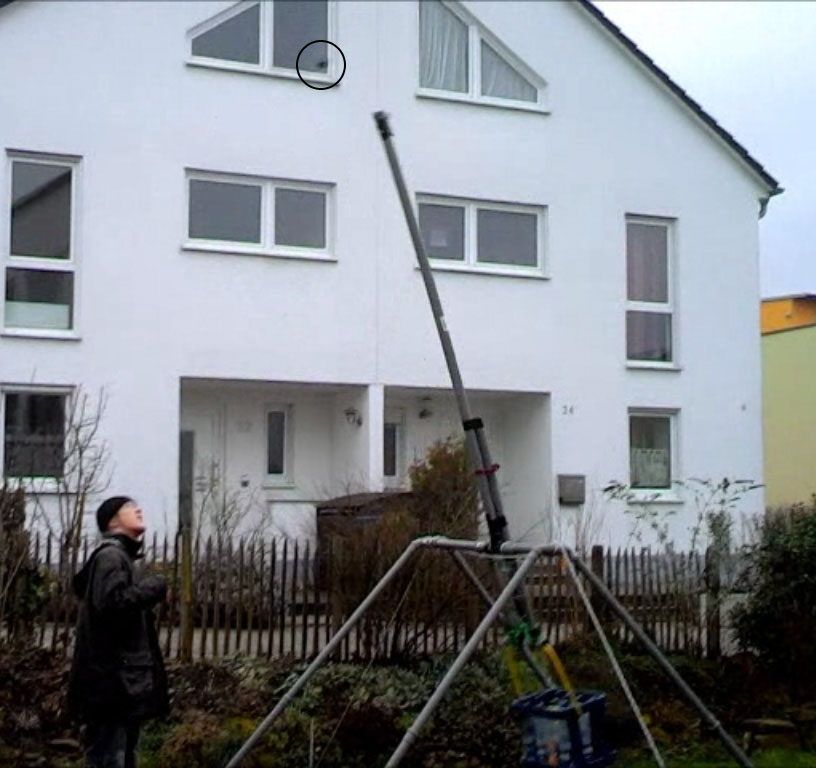
\includegraphics[width=\textwidth]{bilder/tech}
    \caption{Das Trebuchet in Aktion.}
\end{figure}

\section{Aufbau}
Das von mir gebaute Trebuchet besteht aus zwei 1 m langen PVC-Rohren (4 cm Durchmesser) auf allen vier Seiten, wobei jeweils vier Rohre über zwei $45^\circ$-Stücke und ein T-Stück verbunden sind (siehe Bild).  Die zwei T-Stücke sind über die Drehachse miteinander verbunden und werden durch zwei Abspannseile gesichert. Die Achse befindet sich in etwa 1,5 m Höhe und ist 1 m lang, ihre Biegefestigkeit wird durch im Innern liegende Holzstäbe verbessert. Der Hebelarm besteht aus einem 2 m langen Rohr als Wurfarm und zwei 44 cm langen Rohren als Gegengewichtsarm, an dessen Ende mit einem Gartenschlauch ein gefüllter Getränkekasten (Gewicht 1-18 Kg, je nach Anzahl der Flaschen) befestigt ist. Diese drei Rohre sind über drei T-Stücke miteinander verbunden, die Rohre des Hebelarmes und die T-Stücke haben einen größeren Innendurchmesser als die Achse, um drehbar zu sein. Des weiteren ist der Wurfarm mit dem Gegengewichtsarm über ein 1 m langes Rohr verbunden, da die T-Stücke allein nicht verwindungssteif sind.

Das Geschoss ist ein Golfball, der mit Drachenschnur an einem Haken am Ende des Wurfarmes hängt.

\begin{framed}
Technische Daten

$\varphi_{lk}=\frac{3\pi}{4}$, 
$\varphi_P=\frac{\pi}{4}$

$m_G=12\unit{Kg}$, 
$m_{lk}=1.75\unit{Kg}$, 
$m_P=44\unit{g}$

$r_k=44\unit{cm}$, 
$r_l=2\unit{m}$,
$r_P=2.1\unit{cm}$, 
$b=4\unit{cm}$
\end{framed}

\section{Durchführung}
Um das Geschoss abzuschießen, wird der Wurfarm nach unten gedrückt oder das Gegengewicht angehoben. Dann wird die Schlaufe der Schnur, an der der Golfball hängt, an einen Haken am Ende des Wurfarmes eingehängt. Die Länge der Schnur und der Winkel des Hakens bestimmen den Abwurfwinkel. Schließlich wird der Wurfarm freigegeben und das Geschoss wird geworfen. Ein Video zur Demonstration ist im Internet unter \url{http://goo.gl/lE9gR} zu finden.





\section{Ergebnisse}
Die maximale Reichweite des Trebuchets liegt nach einigen Testläufen mit 12 Kg Gegengewicht bei 49 m. Einsetzen der realen Werte meines Trebuchets in (\ref{reichweite}) ergibt folgendes\footnote{Der Faktor $\varsigma$ muss natürlich angepasst werden, denn der Wurfarm kann bis auf $-45^\circ$ heruntergezogen werden, wie dem Bild zu entnehmen ist: 
$\frac{ \frac{
 		\int_
 			{-\frac{\pi}{4}} ^\frac{\pi}{2} 
 			\cos{\varphi}\mathrm d\varphi}{
 			\frac{3\pi}{4}
 		} +
 		 \frac{
 		\int_
 			{-\frac{\pi}{4}} ^0
 			\cos{\varphi}\mathrm d\varphi
 		}{
 			\frac{\pi}{4}
 		}}{2}\approx 0.81 $
}:
\begin{align*}
s &= 2 \varphi_{lk} \varsigma \sin{(2\varphi_P)} \ \ \frac{ m_G  r_kr_l^2}
		{m_{lk} \frac{r^2+b^2}{12} + m_{lk} (\frac{3r_k-r_l}{2})^2+m_P r_l^2}\\
		&=2\cdot \frac{3\pi}{4} \cdot 0.81 \frac{ 12\unit{Kg}\cdot 0.44\unit{m}\cdot (2\unit{m})^2}
		{1.75\unit{Kg} \cdot\frac{(2.44\unit{m})^2+(0.04\unit{m})^2}{12} + 1.75\unit{Kg} \cdot(\frac{3\cdot0.44\unit{m}-2\unit{m}}{2})^2+0.044\unit{Kg} \cdot(2\unit{m})^2}\\
		&\doteq 65 \unit{m}
\end{align*}
Die Abweichung von ca. 25\% ist auf den nicht perfekten Abwurfwinkel, die Vereinfachung in (\ref{bewegungsgleichung_i}) und vor allem auf die Reibungsverluste durch die Achse zurückzuführen. Der Luftwiederstand und der Federeffekt (siehe Bild) des Hebelarms spielen auch eine nicht unerhebliche Rolle.

Der Luftwiderstand des Geschosses hingegen ist kein Faktor, der die Reichweite meines Trebuchets stark beeinflusst, denn der Golfball ist recht aerodynamisch und die maximale Geschwindigkeit des Geschosses (etwa 20 m/s) ist gering. Die Stokes'sche Reibung des Balles ist mit maximal $F_R=6\pi r_P v_{max}\cdot1.9\cdot10^{-5}\unit{Pa\ s}\doteq1.5\cdot10^{-4}\unit{N}$ vernachlässigbar gering.

Zwar ist die Abweichung recht groß, aber wenn man bedenkt, dass die Formel weder die Reibungsverluste an der Achse noch den Luftwiderstand des Hebelarms berücksichtigt, ist sie trotzdem eine gute Abschätzung für die Reichweite.